\documentclass{article}
\usepackage{graphicx} % Required for inserting images
\usepackage{caption}
\usepackage{float}
\usepackage[T1]{fontenc} % Enable guillemets and better font encoding
\usepackage[table]{xcolor} % Enable \rowcolor for tables
\usepackage{hyperref}


\title{\textbf{Relazione Progetto di Tecnologie Web}}
\date{}


\newcommand{\componenti}{
    & Enrico Bianchi - 2040978 - enrico.bianchi.4@studenti.unipd.it\\
    & Davide Martinelli - 2077679 - davide.martinelli.1@studenti.unipd.it \\
    & Marco Cola - 2079237 - marco.cola.1@studenti.unipd.it\\
    & Riccardo Valerio - 2075517 -riccardo.valerio@studenti.unipd.it\\
}
\renewcommand{\contentsname}{Indice}


\begin{document}
\maketitle

\begin{figure}[H]
    \centering
    
\includegraphics[width=0.4\textwidth]{img/logo_unipd.png}
    \label{fig:logo_unipd}
\end{figure}

\vspace{0.5cm}

\begin{center}
\begin{tabular}{r|l}
    \textbf{Componenti} \componenti 
\end{tabular}

\vspace{1cm}
\rule{\linewidth}{0.2mm}

\vspace{0.3cm}

\textbf{Informazioni sul sito} \\
\textbf{Indirizzo sito web:} tecweb.studenti.math.unipd.it/damartin \\
\textbf{Email referente del gruppo: }davide.martinelli.1@studenti.unipd.it

\vspace{0.3cm}
\rule{\linewidth}{0.2mm}

\vspace{0.5cm}
\textbf{Accessi predisposti al sito}
\begin{table}[h]
    \centering
    \begin{tabular}{|p{5cm}|p{5cm}|}
        \hline
        \rowcolor{gray!30}
        Nome utente & Password \\
        \hline
        admin & admin   \\
        \hline
        user & user   \\
        \hline
    \end{tabular}
\end{table}

\end{center}

\newpage

\tableofcontents        %indice

\newpage

\section{Introduzione}
La \textbf{Biblioteca Luzzatti} è una biblioteca universitaria situata in Via Luzzatti 8, nel cuore di Padova, a pochi minuti dall'aula \textbf{LUM250}. La biblioteca rappresenta da anni un punto di riferimento per studenti, docenti e appassionati di lettura, offrendo un ambiente accogliente e una vasta collezione di volumi accessibili a tutta la comunità accademica.

Per supportare e ampliare i servizi offerti, è stato sviluppato un sito web dedicato alla biblioteca, pensato per migliorare l'esperienza di consultazione e rendere più semplice l'interazione con il catalogo. Il portale nasce con obiettivi chiari:

\begin{itemize}
    \item Offrire un'interfaccia semplice, intuitiva e accessibile per permettere agli utenti di esplorare facilmente il catalogo disponibile;
    \item Semplificare e velocizzare la gestione del patrimonio librario tramite un'area riservata pensata per bibliotecari e amministratori, con strumenti per aggiungere, aggiornare e rimuovere titoli in autonomia;
    \item Garantire una navigazione fluida e coerente sia da dispositivi desktop che da smartphone e tablet, grazie a un design responsive e accessibile.
\end{itemize}

Il sito non si limita a fornire un elenco di volumi, ma vuole essere un vero e proprio spazio digitale dove gli utenti possono creare wishlist personalizzate, scrivere recensioni, consultare le esperienze degli altri lettori e contribuire attivamente alla vita della biblioteca.

Questo documento descrive nel dettaglio le scelte progettuali, le funzionalità implementate e le soluzioni tecnologiche adottate per lo sviluppo del sito, con particolare attenzione alla qualità dell'esperienza utente, all'accessibilità e alla semplicità di manutenzione.


\newpage

\section{Analisi dei requisiti}
Per progettare un sito efficace e realmente utile agli utenti, il team ha condotto un'attenta raccolta dei requisiti attraverso diverse modalità. Sono stati realizzati colloqui diretti con i bibliotecari per comprendere le esigenze e le priorità nella gestione del catalogo. Parallelamente, sono stati somministrati questionari anonimi a studenti dell'Università per raccogliere opinioni sulle funzionalità desiderate, sulle abitudini di navigazione e sulle criticità riscontrate in esperienze simili.
A completamento dell'analisi, è stato effettuato un confronto strutturato con portali accademici già esistenti per identificare best practice in termini di organizzazione, accessibilità e velocità di consultazione.
Durante tutto il processo, sono stati considerati come obiettivi prioritari:

\begin{itemize}
    \item Un'elevata accessibilità per rendere il sito fruibile da parte di tutti, compresi utenti con disabilità.
    \item Tempi di risposta rapidi.
    \item Una facilità di manutenzione per consentire di aggiornare rapidamente i contenuti senza particolari complessità tecniche.
\end{itemize}


\subsection{Tipi di utenti}
Il sistema distingue tre principali categorie di utenti, ognuna con permessi e funzionalità differenti:
\begin{itemize}
    \item \textbf{Visitatore (utente anonimo)} - può navigare liberamente il sito, consultare il catalogo, visualizzare le schede dettagliate dei libri, conoscere gli orari di apertura e accedere alle informazioni generali sulla biblioteca e sui servizi offerti.  
    \item \textbf{Utente registrato} - dispone delle funzionalità accessibili ai visitatori, ma ha anche la possibilità di:
          \begin{itemize}
              \item Creare e gestire una wishlist personale per organizzare i libri di interesse;
              \item Inserire recensioni e valutazioni per condividere opinioni con la comunità;
              \item Accedere alla propria cronologia, che include le wishlist passate e le recensioni scritte.
          \end{itemize}
    \item \textbf{Amministratore / Bibliotecario} - oltre alle funzionalità standard, può accedere a una dashboard di gestione per:
          \begin{itemize}
              \item Eseguire operazioni di aggiunta, modifica, eliminazione e visualizzazione dei libri nel catalogo (CRUD);
              \item Eliminare le recensioni pubblicate dagli utenti per garantire la qualità e la pertinenza dei contenuti;
          \end{itemize}
\end{itemize}


\subsection{Funzionalità}
Il sito è progettato per offrire agli utenti un set di funzionalità complete e intuitive:
\begin{itemize}
    \item \textbf{Sistema di ricerca avanzata} con filtri per titolo, genere e autore, rapido e facilmente accessibile dalla pagina catalogo;
    \item \textbf{Schede libro} dettagliate, complete di trama, dati editoriali, immagine di copertina e recensioni;
    \item Possibilità per gli utenti registrati di gestire \textbf{wishlist e recensioni personali} direttamente dal proprio profilo;
    \item \textbf{Area riservata} per accedere a funzionalità personalizzate e visualizzare la cronologia delle attività;
    \item \textbf{Dashboard amministrativa} dedicata alla gestione dei contenuti e alla moderazione delle recensioni;
    \item \textbf{Design responsive e accessibile}, pienamente compatibile con dispositivi mobili e conforme alle linee guida WCAG 2.2 livello AA, per garantire un'esperienza inclusiva e coerente su qualsiasi piattaforma;
    \item Disponibilità di un \textbf{layout di stampa ottimizzato} per consentire agli utenti di stampare schede e contenuti in modo ordinato e leggibile.
\end{itemize}


\section{Progettazione}
La progettazione del sito web è stata sviluppata con l'obiettivo di creare un'esperienza utente semplice, intuitiva e accessibile, in grado di sottolineare i servizi offerti dalla biblioteca e di facilitare la navigazione del catalogo da parte di utenti con diversi livelli di familiarità con le tecnologie digitali.
Ogni sezione è stata pensata per offrire contenuti chiari, strutturati e facilmente navigabili.


\subsection{Schema organizzativo}
Il sito si articola in quattro sezioni principali: \emph{\textbf{Home}}, \emph{\textbf{Chi siamo}}, \emph{\textbf{Catalogo}} e \emph{\textbf{Area riservata}}.  
Nella Home vengono presentate la missione della biblioteca, i servizi offerti, i contatti e gli orari.  
La pagina “Chi siamo” è suddivisa in blocchi dedicati alla missione, alla storia tramite una timeline interattiva, alla presentazione del team e alle modalità di contatto con mappa incorporata.  
Il Catalogo mostra visivamente i libri disponibili (copertina, titolo, autore, genere e breve descrizione) e offre una ricerca live per filtrare i risultati.  
L’Area riservata prevede un login/registrazione: gli utenti possono gestire wishlist e recensioni, mentre admin e bibliotecari hanno accesso a un cruscotto per aggiornare il catalogo e i contenuti del sito.

\subsection{Visibilità “Above the Fold”}
In tutte le pagine l’altezza dei contenitori principali è studiata per mantenere i contenuti chiave “above the fold”. Gli elementi si navigano tramite:
\begin{itemize}
  \item frecce e indicatori cliccabili col mouse  
  \item frecce direzionali e Tab per la tastiera  
  \item swipe su dispositivi touch  
\end{itemize}


\newpage

\section{Organizzazione e Suddivisione del lavoro}
Il lavoro è stato suddiviso come segue:
\begin{itemize}
    \item \textbf{Davide Martinelli}:
            \begin{itemize}
                \item sviluppo del design e comportamento del catalogo;
                \item design e sviluppo della funzionalità recensioni;
                \item testing di accessibilità;
                \item validazione HTML/CSS, contrast-checker;
                \item supporto layout di stampa;
                \item scrittura della relazione progettuale.
            \end{itemize}
    \item \textbf{Marco Cola}:
            \begin{itemize}
                \item realizzazione template HTML5 semantici;
                \item miglioramento stile e struttura CSS;
                \item progettazione schema database;
                \item scrittura della relazione progettuale.
            \end{itemize}
    \item \textbf{Enrico Bianchi} :
            \begin{itemize}
                \item progettazione/realizzazione database e interazione tramite PHP;
                \item sviluppo di script JavaScript per la validazione dei dati client-side e visualizzazione degli errori;
                \item sviluppo di script PHP per la validazione dei dati server-side, salvataggio su database e visualizzazione errori;
                \item controllo degli elementi dei form per verirficare l’uso corretto degli attributi di accessibilità;
                \item scrittura della relazione progettuale.
            \end{itemize}
   \item \textbf{Riccardo Valerio}:
            \begin{itemize}
                \item implementazione HTML;
                \item implementazione della struttura e dello stile CSS;
                \item validazione HTML/CSS;
                \item popolamento del database;
                \item scrittura della relazione progettuale.
            \end{itemize}
\end{itemize}


\newpage

\section{Implementazione Front-End}

\subsection{Struttura delle Pagine (HTML)}

Il sito web della \textbf{Biblioteca Luzzatti} è stato progettato con un'architettura HTML5 modulare, accessibile e semanticamente coerente. Ogni pagina adotta una struttura uniforme composta da elementi ricorrenti:

\begin{center}
\texttt{<header> - <nav> - <main> - <footer>}
\end{center}

L'intestazione (\texttt{<header>}) contiene il logo della biblioteca ed è accompagnata da un menu di navigazione adattivo: nelle visualizzazioni su dispositivi mobili si trasforma in un menu “hamburger”. Il menu mostra voci diverse in base allo stato dell’utente (anonimo, autenticato o amministratore), e la voce relativa alla pagina corrente non è cliccabile.

Il contenuto principale è racchiuso in \texttt{<main id="contenuto">}, con le informazioni organizzate in \texttt{<section>}, e arricchite da placeholder che vengono sostituiti dinamicamente lato server tramite PHP.

Ogni pagina, eccetto l’homepage e la pagina di errore, presenta un \texttt{breadcrumb} che migliora la tracciabilità della posizione corrente e consente una navigazione gerarchica semplificata.

Il piè di pagina (\texttt{<footer>}) è presente su tutte le pagine e include i recapiti, gli orari e link ai canali social. In fondo a ogni documento è inserito un pulsante “Torna su” per facilitare la navigazione da tastiera.

Infine, tutte le pagine sono valide secondo lo standard W3C, scritte in HTML conforme alla sintassi XML e testate per garantire compatibilità e accessibilità su tutti i dispositivi.

\medskip

\noindent
\textbf{Aspetti di accessibilità e SEO}:
\begin{itemize}
    \item Uso sistematico di landmark semantici (\texttt{<header>}, \texttt{<nav>}, \texttt{<main>}, \texttt{<footer>}).
    \item Titoli gerarchici, link descrittivi e immagini con \texttt{alt} significativo.
    \item Navigazione da tastiera completa.
    \item URL descrittivi e contenuti ottimizzati per l’indicizzazione nei motori di ricerca.
\end{itemize}

\vspace{1em}

\subsection{Design e Styling (CSS)}

Lo stile grafico del sito è stato realizzato interamente a mano, tramite un unico foglio CSS centrale (\texttt{style.css}).

\medskip

\noindent
\textbf{Caratteristiche principali dello stile:}
\begin{itemize}
    \item \textbf{Modularità e coerenza}: l’uso di variabili globali definite con \texttt{:root} (es. \texttt{--headerbgcolor}, \texttt{--txtcolor}) consente di mantenere un’identità visiva uniforme.
    \item \textbf{Layout responsive}: il sito impiega sia \textbf{Flexbox} sia \textbf{CSS Grid} per la disposizione dei contenuti, garantendo adattabilità a ogni tipo di dispositivo. Le sezioni principali si adattano dinamicamente alla larghezza dello schermo e il menu diventa hamburger sotto una certa dimensione.
    \item \textbf{Contrasto e accessibilità visiva}: i colori sono scelti per garantire un contrasto minimo AA (WCAG 2.2), e tutti gli elementi interattivi prevedono stati \texttt{:hover} e \texttt{:focus} ben visibili.
    \item \textbf{Struttura CSS organizzata}: il foglio di stile è diviso in sezioni (header, breadcrumb, main, footer, tabelle, errori, form, ecc.) per facilitarne la manutenzione e l’estensione futura.
\end{itemize}

\medskip

Questa organizzazione permette una netta separazione tra contenuto (HTML), presentazione (CSS) e comportamento (PHP/JS), in linea con i principi richiesti dal progetto.

\subsection{Convenzioni interne}
Nello sviluppo del sito sono state definite alcune convenzioni utili a una corretta navigazione:
\begin{itemize}
    \item link non visitati di colore rosso;
    \item link visitati di colore nero;
    \item nome dell'informazioni di libri e recensioni di colore blu e dentro un tag \texttt{<strong>};
    \item bottoni di eliminazione libri dalla wishlist e recensioni di colore rosso con icona apposita e \texttt{label} ad hoc.
\end{itemize}




\subsection{Dinamismo e Interazione (JavaScript)}
All'interno del sito sono stati utilizzate alcune funzionalità Javascript, in particolare per la validazione lato client dei form. Di seguito si elencano i rispettivi impieghi.
Il file \texttt{script.js} gestisce:
\begin{itemize}
    \item apertura e chiusura del menu verticale;
    \item alterna lo stato visibile del menu e delle relative icone;
    \item controlla se il menu è aperto o chiuso e cambia di conseguenza.
\end{itemize}

Invece il file \texttt{val\_reg.js} gestisce:

\begin{itemize}
    \item validazione dei dati inseriti all'interno del form di registrazione con conseguente visualizzazione degli errori se necessaria;
    \item validazione dei dati inseriti all'interno del form aggiunta/modifica di un libro da parte dell'admin con conseguente visualizzazione degli errori se necessaria;
    \item validazione dei dati inseriti all'interno del form di recensione con conseguente visualizzazione degli errori se necessaria;
    \item impedisce l'invio di un form nel caso siano presenti errori;
    \item Rimuove automaticamente spazi all'inizio/fine di password e conferma password durante la digitazione.
\end{itemize}



\subsection{Gestione della Stampa e dei Media (CSS per Stampa)}
Per quanto riguarda il layout di stampa delle varie pagine del sito sono state adottate delle scelte che mirano a inserire nel foglio da stampare solo le informazioni veramente importanti. Le regole css di stampa sono definite nel file \texttt{printstyle.css}. Di seguto vengono descritte:
\begin{itemize}
    \item Vengono eliminate la totalità delle immagini e delle mappe per evitare spreco di inchiostro;
    \item Lo stile della pagina originale viene ridotto al minimo riportando solo informazioni testuali in bianco e nero;
    \item Viene totalmente eliminato il footer essendoci la pagina "Chi siamo" che ricopre lo stesso scopo;
    \item Oltre al contenuto essenziale della pagina rimane anche il titolo del sito e l'elenco ordinato del breadcrumb.
\end{itemize}

\newpage


\section{Implementazioni back-end}



\subsection{JavaScript}

Javascript è stato utilizzato per la gestione del menu verticale e per la validazione dei dati lato client.
Attraverso la manipolazione del DOM, ogni modifica a un campo di input di un form (rilevata tramite l'evento \texttt{change}) attiva un controllo sui dati inseriti.
In caso di errori, i messaggi di avviso vengono inseriti all'interno di specifici elementi \texttt{<p>} di classe \texttt{error-msg} dedicati alla visualizzazione degli errori e viene bloccata la possibilità di \texttt{submit} del form.

\subsection{PHP}

PHP è stato utilizzato principalmente per il rendering dinamico delle pagine HTML, gestendo la sostituzione automatica dei segnaposto presenti nei file HTML (solitamente nel formato \#\#\#segnaposto\#\#\# oppure \{\{segnaposto\}\}) con i contenuti appropriati tramite specifici script.

È stata inoltre implementata la validazione lato server dei dati inviati attraverso i form, recuperati utilizzando la variabile globale \texttt{\$\_POST}. Gli eventuali errori di input vengono visualizzati mediante la sostituzione di determinati segnaposti, garantendo così un corretto funzionamento anche nel caso in cui JavaScript sia disabilitato e la validazione lato client con conseguente visualizzazione degli errori non possa essere eseguita.
Nel file \texttt{utils.php} è definita la funzione \texttt{pulisciInput}, pensata per sanificare e normalizzare i dati in ingresso, solitamente provenienti da form HTML, al fine di assicurarne la sicurezza prima di qualsiasi elaborazione o salvataggio.
Il contenuto viene dapprima "ripulito" con \texttt{trim}, che elimina gli spazi bianchi iniziali e finali; successivamente, \texttt{strip\_tags} rimuove qualsiasi tag HTML o PHP potenzialmente dannoso.
Infine, \texttt{htmlentities} converte i caratteri speciali nelle relative entità HTML, evitando che possano essere interpretati come codice eseguibile.
In questo modo, il dato risultante è protetto da vulnerabilità comuni come l'iniezione di codice (XSS).

È stata realizzata la funzione \texttt{check\_session\_timeout}, che consente di terminare automaticamente la sessione utente dopo 30 minuti di inattività sul sito.

Infine, è presente la funzione \texttt{connectDB}, incaricata di stabilire la connessione al database utilizzato. In caso di successo, restituisce un oggetto \texttt{PDO}; in caso contrario, restituisce \texttt{null}.
Nel caso in cui si verifichino errori durante l'interazione con il database, come ad esempio il fallimento nella connessione o l'esecuzione non riuscita di una query, l'utente viene reindirizzato alla pagina \texttt{505.php}.
\subsection{Database}
Il database è stato progettato per la gestione di una biblioteca digitale e comprende tabelle relative a utenti, libri e interazioni come recensioni e wishlist.

\begin{itemize}
    \item \textbf{Clienti}: contiene le informazioni degli utenti registrati. Ogni cliente è identificato da un campo \texttt{ID\_Cliente} univoco e dispone di un'email, uno username (entrambi univoci), una password e un ruolo. Il ruolo, definito tramite un tipo \texttt{ENUM}, può essere \texttt{Cliente} o \texttt{Admin}, e permette di distinguere tra utenti comuni e amministratori.
    
    \item \textbf{Libri}: memorizza i dettagli dei libri disponibili nel sistema. Ogni libro ha un \texttt{ID\_Libro} univoco, un titolo, un autore, un'immagine di copertina (\texttt{Image\_path}), la casa editrice, il genere, l'anno di pubblicazione e una descrizione della trama.
    
    \item \textbf{Wishlist}: rappresenta una relazione molti-a-molti tra clienti e libri. Ogni record indica che un certo cliente ha aggiunto un determinato libro alla propria lista dei desideri. La chiave primaria è composta dalla coppia \texttt{(Cliente, Libro)}. I vincoli di chiave esterna assicurano l'integrità referenziale con le tabelle \texttt{Clienti} e \texttt{Libri}.
    
    \item \textbf{Recensioni}: consente ai clienti di lasciare una valutazione e una recensione testuale per ciascun libro. Ogni recensione è associata a un cliente e a un libro, e contiene anche la data di inserimento (\texttt{Data}). Anche qui la chiave primaria è composta da \texttt{(Cliente, Libro)}, garantendo una sola recensione per libro da parte di ogni utente.
\end{itemize}

Il database viene inizialmente popolato con dieci libri di generi diversi, completi di informazioni bibliografiche, immagini di copertina e trame dettagliate.

\newpage
\section{Accessibilità}
Il sito mira ad essere completamente accessibile al livello \textbf{AA} delle WCAG 2.2. 
\subsection{Validazione HTML5}
I primi test effettuati sono stai fatti tramite l'app HTML validator Basic, a cui è stata sottoposta sia la validazione di livello AA sia AAA. Tutte le pagine non risultano avere alcun errore a parte le seguenti eccezioni:
\begin{itemize}
    \item Warning di mancanza di un link di "skip-navigation" - avvertenza generata da un falso positivo: infatti il link è presente non appena inizia il tag \texttt{body};
    \item Warning di mancanza degli alt nelle immagini - alcuni alt di immagini presenti nel sito, ovvero quelli relativi alle immagini di copertina dei libri, sono vuoti poichè abbiamo considerato che queste immagini svolgessero un semplice ruolo decorativo, pertanto esse sono prive di una descrizione alternativa.
\end{itemize}

In seguito ai test eseguiti con HTML Validator Basic, sono stati svolti alcuni test, più semplici e veloci, con l'estensione silktide e Wave con il livello di accessibilità AA. Dalle appena citate estensioni non sono pervenuti errori se non uno sul form di ricerca dei libri nella pagina di catalogo: Silktide considera i contrasti troppo lievi, cosa che controllando manualmente e con l'utilizzo di altri strumenti non ci risulta. Il colore del form, pertanto, non subisce variazioni.

\subsection{Validazione CSS}
Il CSS è stato validato con lo strumento messo a disposizione da w3c, \url{https://jigsaw.w3.org/css-validator/}, con esito positivo.

\subsection{Contrasti}
Oltre ai controlli effettuati con le estensioni Silktide e Wave sono stati effettuati controlli ad hoc anche con l'estensione WCAG Contrast checker. Il livello imposto a questa estensione è stato AA. I test effettuati con questo strumento, senza l'utilizzo di filtri, sono stati passati con successo. Riportiamo inoltre che con i filtri "tritanopia" e "deuteranopia" presentano lievi errori. Di seguito si allegano alcuni esempi dell'appena descritta analisi dei contrasti.

\vspace{1cm}

\begin{figure}[H]
    \begin{minipage}[t]{0.5\textwidth}
        \centering
        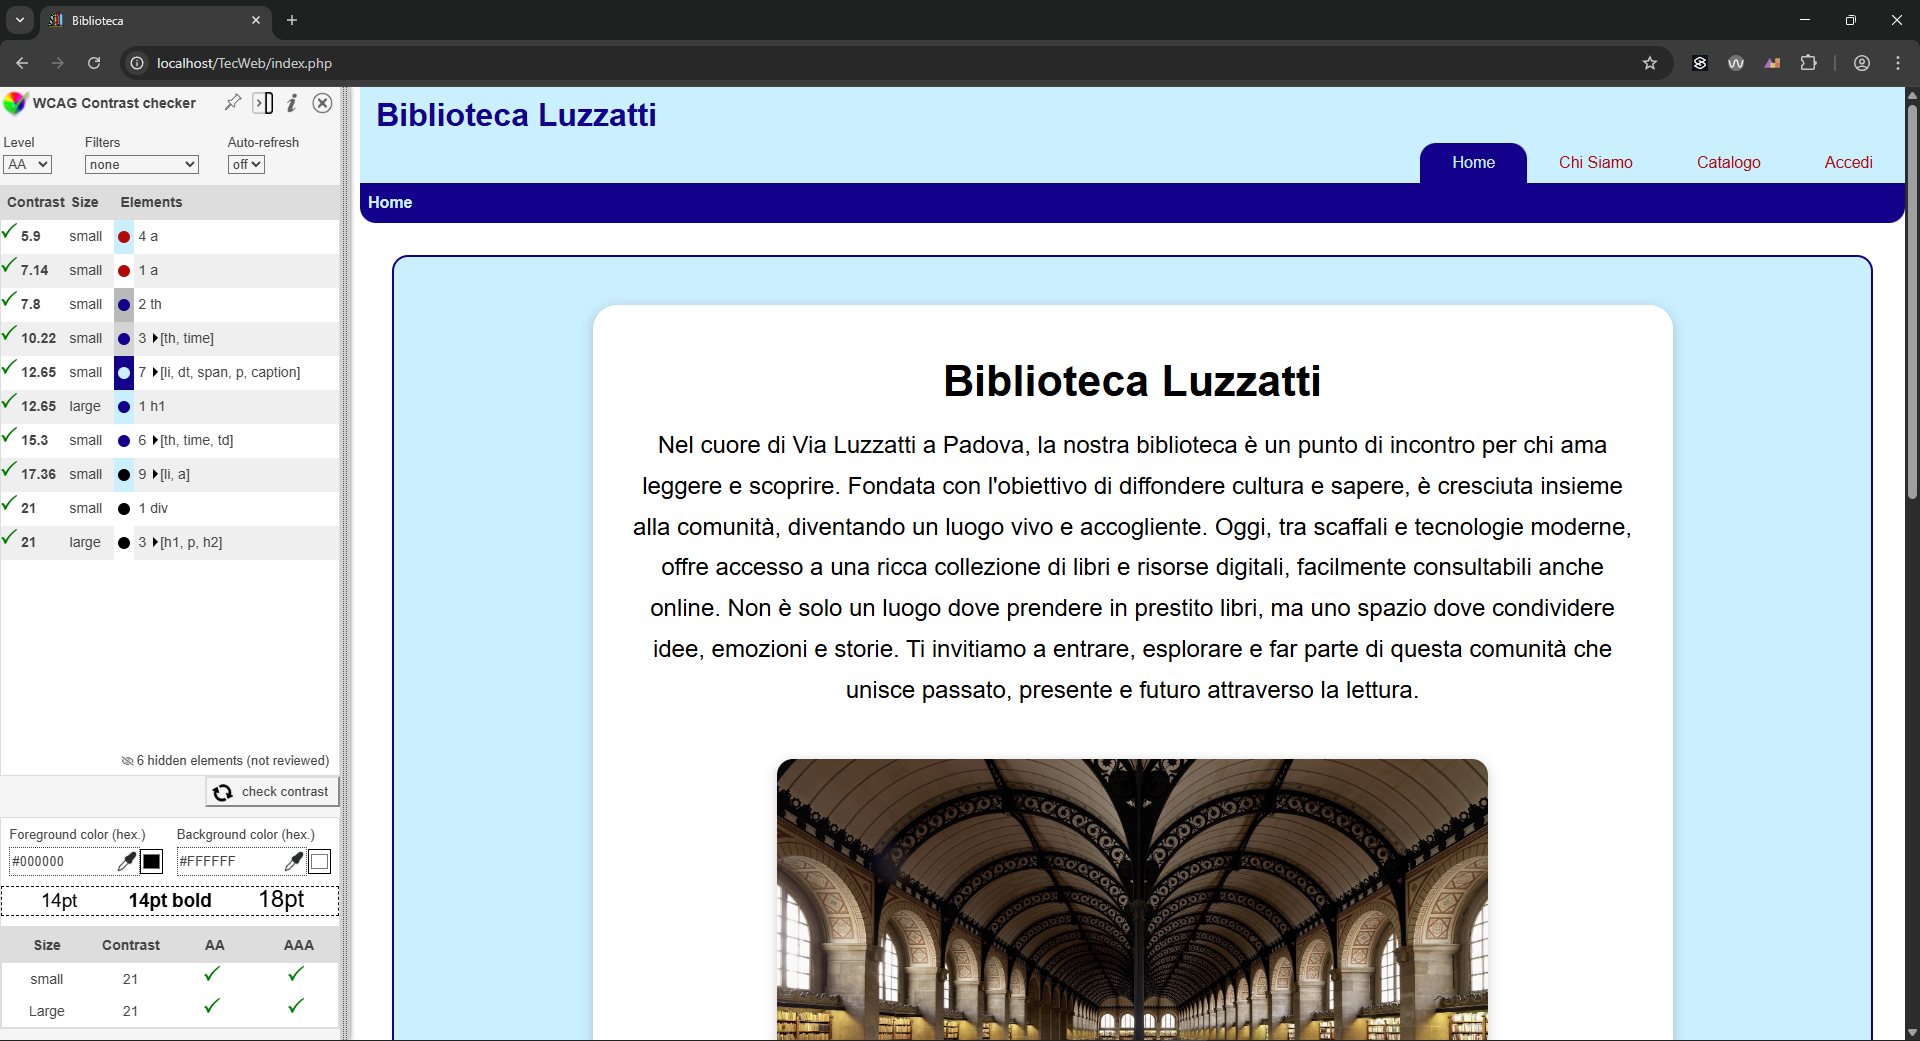
\includegraphics[width=\textwidth]{./img/home.png}
        \caption{Home}
    \end{minipage}
    \hfill
    \begin{minipage}[t]{0.5\textwidth}
        \centering
        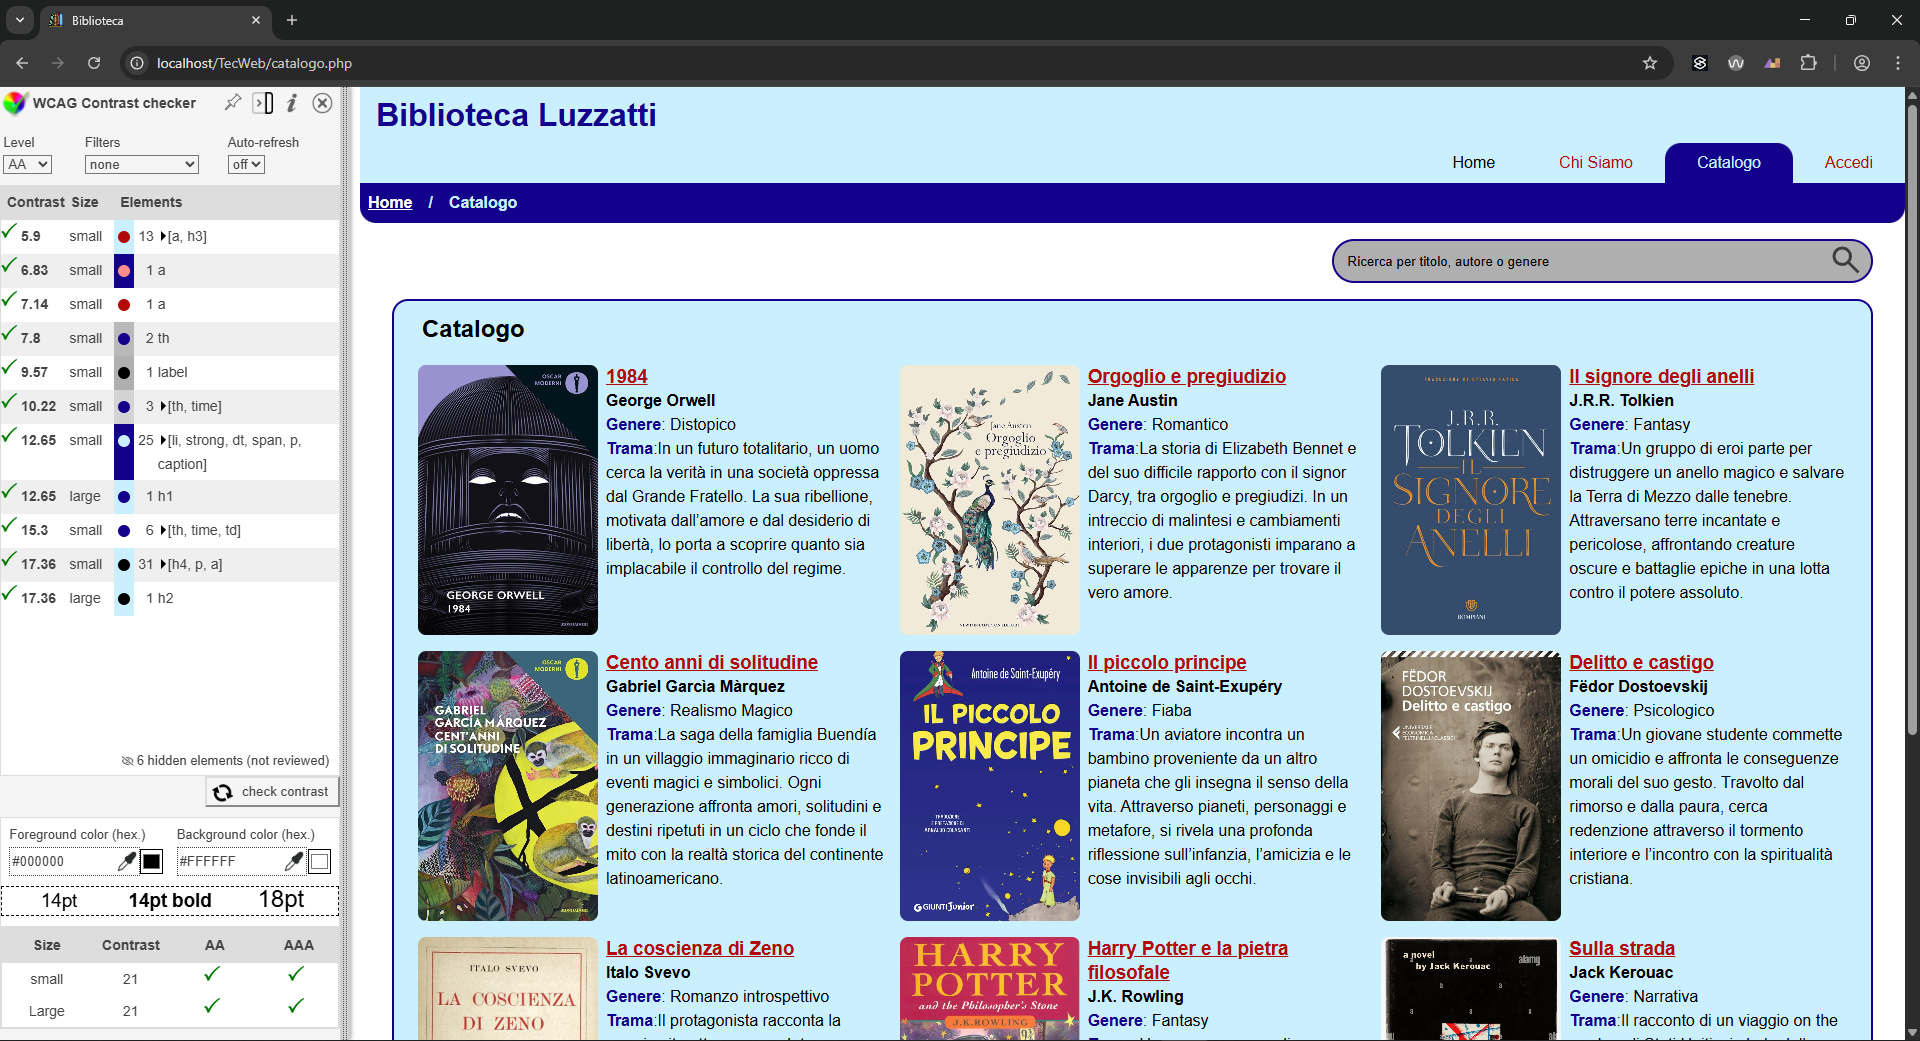
\includegraphics[width=\textwidth]{./img/catalogo.png}
        \caption{Catalogo}
    \end{minipage}
    \hfill
    \begin{minipage}[t]{0.5\textwidth}
        \centering
        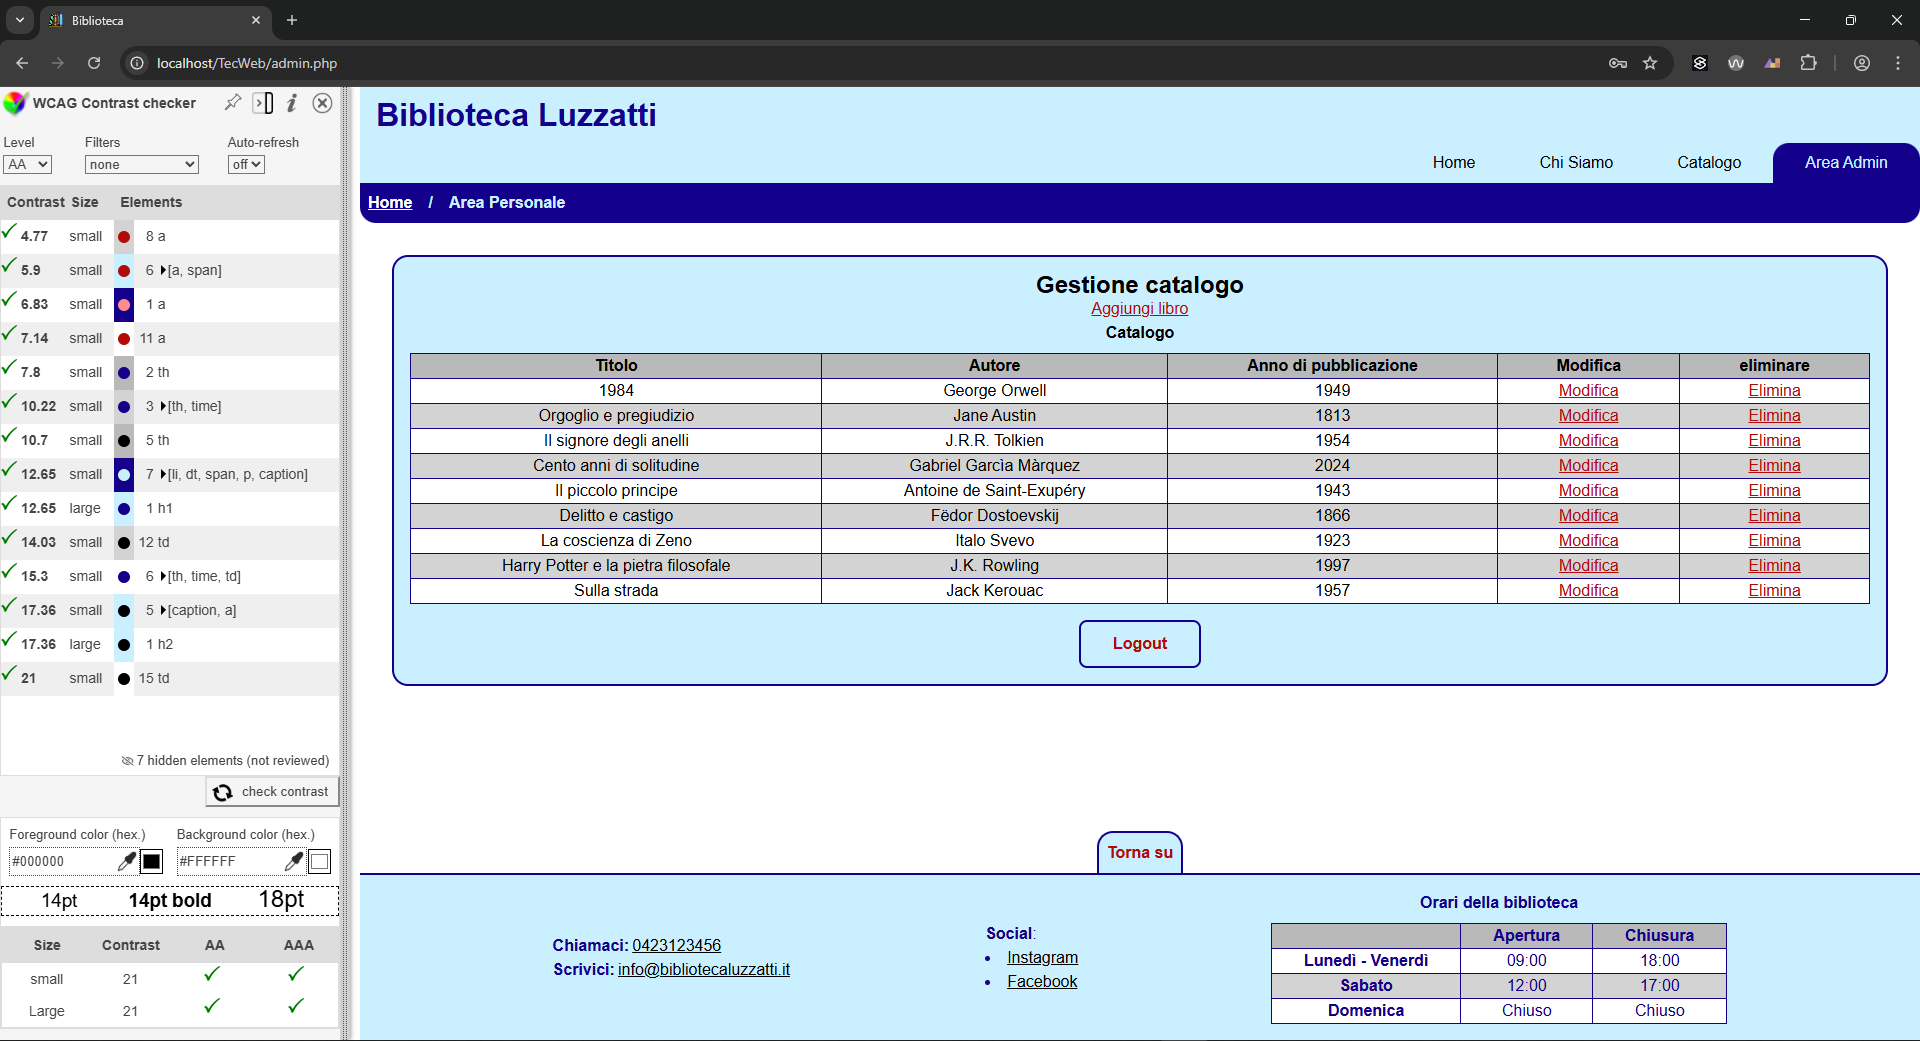
\includegraphics[width=\textwidth]{./img/admin.png}
        \caption{Admin}
    \end{minipage}
    \hfill
    \begin{minipage}[t]{0.5\textwidth}
        \centering
        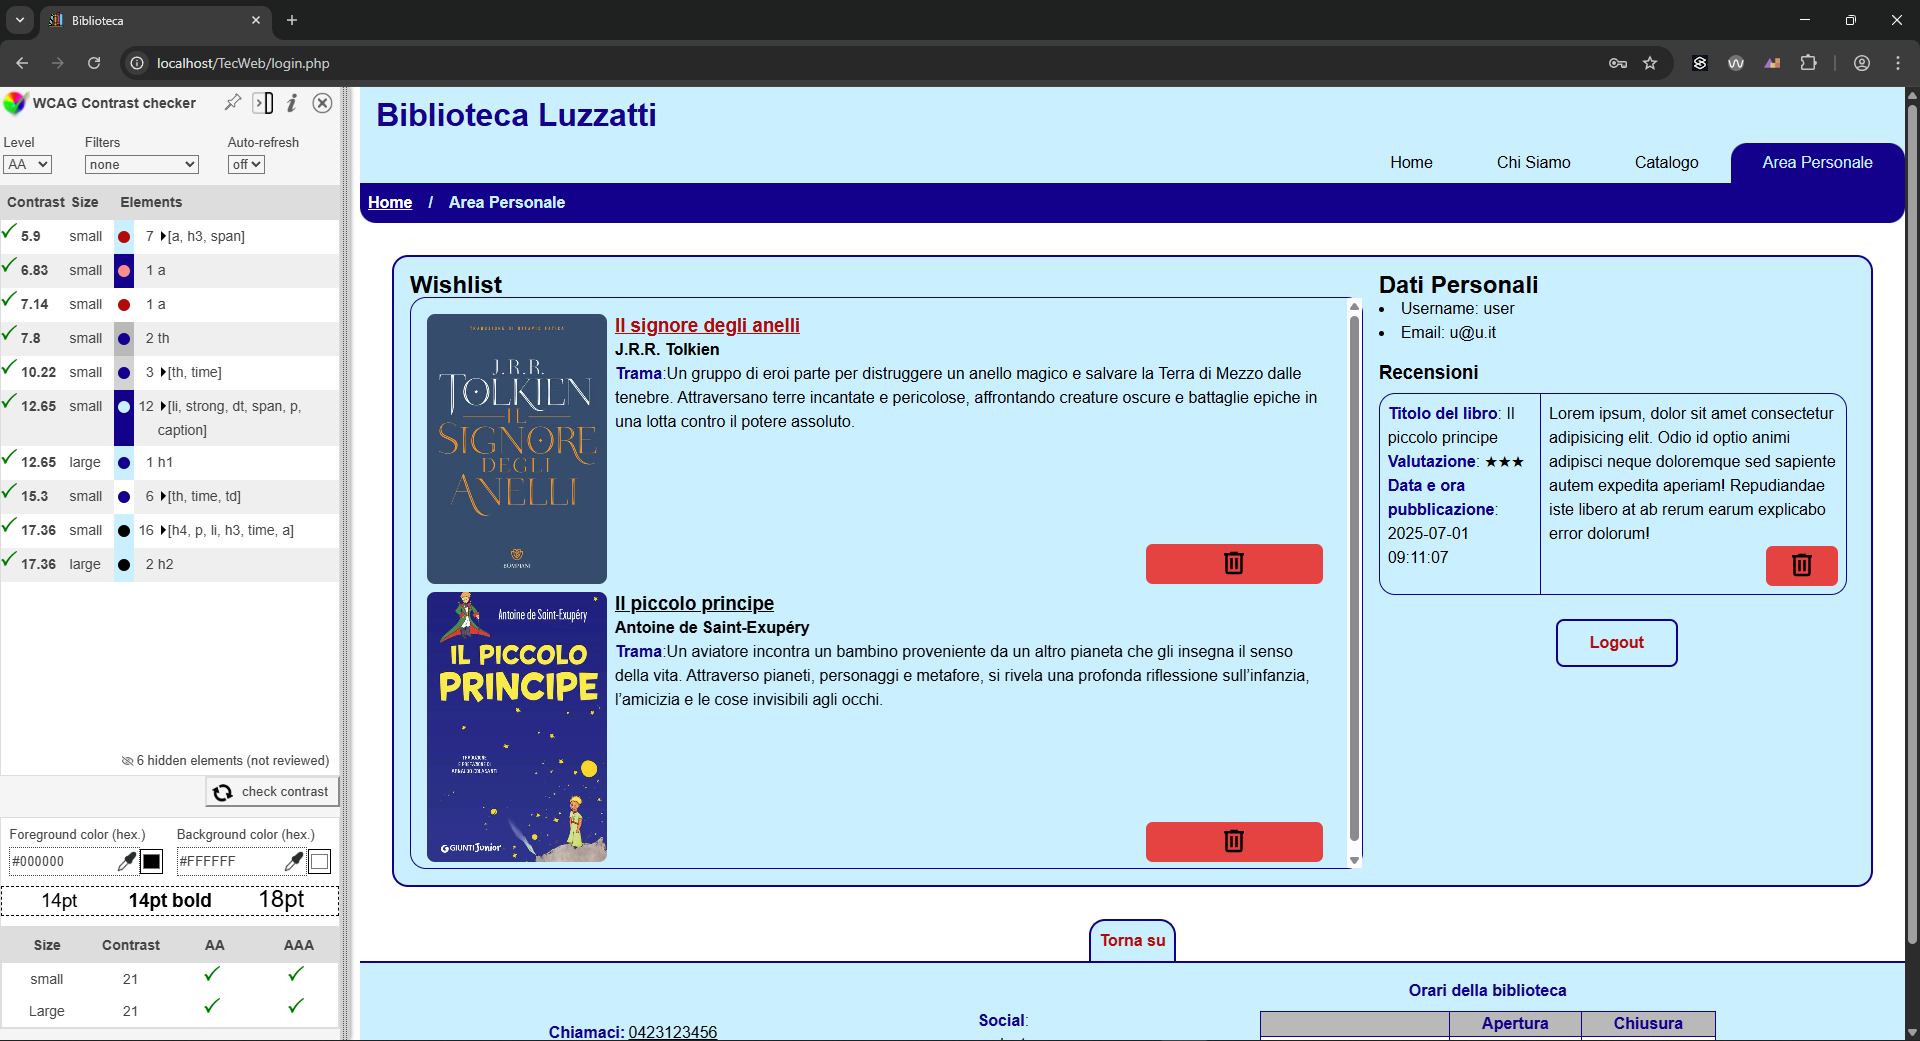
\includegraphics[width=\textwidth]{./img/area_riservata.png}
        \caption{Area riservata}
    \end{minipage}
\end{figure}


\subsection{Screen Reader}
Per completare l'analisi di accessibilità del sito, esso viene sottoposto a vari test tramite l'utilizzo di screen reader. Il sito è stato sottoposto a test con lo screen reader di Silktide e uno screen reader esterno al browser: NVDA. Nel corso della navigazione nel sito essi non hanno trovato alcuna difficoltà.

\end{document}